\begin{problem}{개선문}
	{standard input}{standard output}
	{1 second}{128 megabytes}{}
	
	
	Byteotia의 왕인 Byteasar은 전투를 승리로 이끌고 나라로 돌아오고 있다. Byteotia에는 $n-1$개의 도로로 연결된 $n$개의 도시가 있다. 모든 도시는 다른 도시까지 하나보다 많은 도로를 거쳐서 가는 유일한 경로가 존재한다. (다른 말로, 도로망은 트리 형태이다.)
	
	왕이 방금 수도로 들어왔다. 수도에는 전쟁에서 승리한 왕을 기리는 개선문이 건설되었다. 열렬한 환영에 감동한 Byteasar는 자기가 현재 있는 수도로 부터 시작해 Byteotia에 있는 모든 도시를 방문하는 승리 행렬을 하기로 했다.

	다른 도시는 왕을 반길 준비가 아직 되어있지 않다. 몇몇 도시의 개선문 건설은 시작되지도 않았다! 하지만 Byteasar의 듬직한 조언자는 이 문제를 알고 있다. 그는 요원들을 몇 명 고용하고 싶어 한다. 모든 건설 요원은 어떤 마을이든 하루에 하나씩 개선문을 지을 수 있다. 불행하게도, 아무도 왕이 마을을 방문하는 순서를 모른다. 한가지 확실한 점은 왕은 매일 현재 있는 위치에서 인접한 도시로 여행한다는 것이다. 왕은 어떤 도시든 임의의 횟수만큼 방문할 수 있다. (왕은 허영심이 많지 않기 때문에, 하나에 도시에 하나의 개선문이면 충분할 것이다.)
	
	Byteasar의 조언자는 요원들에게 얼마나 많은 개선문을 짓든 관계 없이 고정된 금액을 주어야 한다. 그리고, 그는 왕이 어떻게 방문하든 모든 위치에 개선문이 있음을 확신함과 동시에, 최소한의 요원들을 고용하고 싶다. 그를 위해 개선문을 제 때 만들기 위해 요원들을 최소로 고용하는 프로그램을 짜는 것을 도와주자.
	
	

	\InputFile
	
	첫째 줄에는, Byteotia의 마을에 수를 나타내는 정수 $n$이 주어진다. ($2 \le n \le 300,000$) 마을은 1번부터 $n$번까지 번호가 붙어있으며, 1번 마을은 수도이다.
	
	다음 $n-1$개의 줄 각각에는 서로 다른 두 정수 $a$와 $b$가 공백 하나로 구분되어 들어온다. 이는 마을 $a$와 $b$를 직접 잇는 양방향 도로가 존재한다는 것이다.
	
	\OutputFile
	
	출력은 한 줄이다. Byteasar의 조언자가 고용해야하는 요원의 수의 최솟값을 출력하여라.
	
	 
	\Examples
		
	\begin{example}
	\exmp{
	7
	1 2
	1 3
	2 5
	2 6
	7 2
	4 1
	}{%
	3
	}%
	\end{example}
    
    첫째 날에 2, 3, 4번 마을에 개선문이 건설되어야 한다. 둘째 날에 5, 6, 7번 마을에 개선문이 건설되어야 한다.
    
    \begin{center}
    	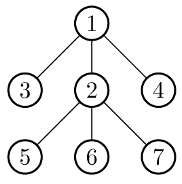
\includegraphics[width=0.23\linewidth]{luk.png}
    \end{center}
        
\end{problem}

